\subsection{1. Introduction}\label{introduction}

Personalization is commonly framed as a memory problem: a user states a
preference, an assistant stores or retrieves it, and evaluation asks
whether the assistant later recalls or follows it. That abstraction
becomes incomplete once preferences evolve, evidence is noisy or
implicit, temporary exceptions occur, and memory is used to trigger
recommendations, reminders, tool actions, or other interventions.

Consider a user who generally prefers morning workouts, temporarily
switches to evenings during a two-week schedule disruption, and later
returns to mornings. A system that always uses the latest apparently
trustworthy fact can be highly accurate on aggregate state queries yet
become overly conservative or overconfident in exactly the cases where
action requires calibrated uncertainty. A second system can maintain a
distribution over plausible current values and decide whether to act or
defer. These systems should not necessarily be judged by the same scalar
recall metric.

This paper studies a stricter evaluation question: \textbf{when
long-horizon personalization drives action, which conclusions survive
changes in calibration protocol and evaluator assumptions?} We formulate
long-horizon personalization as partially observed state estimation
followed by risk-sensitive decision-making. PersonaMetrica-Bench
separates the observation layer from the belief-update layer so the
latter can be stress-tested with known provenance and scope. We then
evaluate both correctness and the relationship between confidence and
downstream action.

Our strongest result is not that one memory algorithm always wins.
Rather, the ranking depends on \textbf{both the metric and the
confidence protocol}. With native confidence, the 800-turn experiment
makes PBS look like a substantially better action substrate despite
slightly lower state accuracy. Once every tracker is given the same
development-only post-hoc calibration opportunity, the fixed-threshold
utility ordering flips and time-aware-latest becomes better at that
operating point. AURC, which depends on confidence ordering rather than
a particular action threshold, still favors PBS. This exposes two
evaluation confounds at once: state accuracy can miss selective-risk
structure, while fixed-threshold utility can reward one system merely
because its confidence scale is better matched to the chosen threshold.

\subsubsection{Contributions}\label{contributions}

\begin{enumerate}
\def\labelenumi{\arabic{enumi}.}
\tightlist
\item
  \textbf{Evaluation framing.} We formalize long-horizon personalization
  as belief-state estimation plus action under uncertainty and argue for
  reporting calibration and risk--coverage alongside state accuracy.
\item
  \textbf{PersonaMetrica-Bench.} A deterministic controlled testbed for
  protocol sensitivity with ten preference domains, durable changes,
  temporary exceptions, explicit/implicit evidence, noisy behavioral
  cues, hypothetical and other-person distractors, long-horizon
  variants, counterfactual interventions, and trajectory-level grader
  stress tests.
\item
  \textbf{Strong executable baselines.} Six memory/state systems ranging
  from first-mention and latest-observation to a time-aware baseline
  that filters distractors and handles temporary expiry.
\item
  \textbf{Personal Belief State.} A transparent evidence-weighted
  temporal representation with provenance, source reliability, recency,
  context scope, expiry, and probabilistic readout.
\item
  \textbf{Evaluation analysis.} Held-out multi-seed statistics,
  risk--coverage/AURC, a threshold/deferral-cost sensitivity sweep, and
  a development-only calibration protocol that reveals when
  native-confidence utility comparisons are not fair.
\item
  \textbf{Evaluator-as-system discipline.} Held-out grader attacks,
  causal trajectory contracts, abstention under missing evidence,
  implementation fingerprints, and disagreement routing test whether the
  measurement system itself generalizes. A 620-item human-annotation
  pack and vendor-neutral external-model evaluator are included as
  unexecuted infrastructure; no human or frontier-model result is
  fabricated.
\end{enumerate}

\subsubsection{Research questions}\label{research-questions}

\begin{itemize}
\tightlist
\item
  \textbf{RQ1 --- Metric sufficiency:} Does state accuracy rank
  personal-state systems the same way as selective risk and downstream
  action quality?
\item
  \textbf{RQ2 --- Calibration fairness:} Do conclusions from
  fixed-threshold utility survive when every system receives the same
  development-only confidence calibration opportunity?
\item
  \textbf{RQ3 --- Mechanism:} Which evidence-handling components of PBS
  account for its behavior under noise, temporary scope, and long
  histories?
\end{itemize}

The paper treats RQ2 as a first-class evaluation question rather than a
post-hoc implementation detail. Any utility comparison that gates action
on confidence is meaningful only relative to an explicit confidence
calibration protocol.

\subsection{2. Problem formulation}\label{problem-formulation}

Let a user have latent preference state \(z_t\). The agent observes
evidence \(x_t\), which may be explicit, implicit, noisy, hypothetical,
about another person, or scoped to a temporary context. A
personalization system maintains a belief

\[
b_t(z)=p(z_t\mid x_{1:t})
\]

and uses it to answer a query or choose an action \(a_t\).

A conventional state metric measures

\[
\mathrm{Acc}=\mathbb{E}[\mathbf{1}(\hat z_t=z_t)].
\]

For an acting assistant this is incomplete. We additionally measure:

\begin{itemize}
\tightlist
\item
  \textbf{coverage:} fraction of queries on which confidence is above an
  action threshold;
\item
  \textbf{selective accuracy:} accuracy conditional on action;
\item
  \textbf{Brier score:} calibration of confidence against correctness;
\item
  \textbf{risk--coverage curve:} error rate as progressively
  less-certain decisions are included;
\item
  \textbf{AURC:} area under the risk--coverage curve, lower is better;
\item
  \textbf{decision utility:} a transparent operating-point metric in
  which correct action is +1, wrong action is −1, and deferral has an
  explicit cost.
\end{itemize}

The utility coefficient is not assumed to be universal. We therefore
report a sensitivity sweep and treat AURC as the more defensible
threshold-free measure of confidence quality.

\subsection{3. Personal Belief State}\label{personal-belief-state}

PBS stores evidence rather than overwriting a single current value. Each
evidence record includes:

\begin{itemize}
\tightlist
\item
  semantic slot and candidate value;
\item
  turn and provenance;
\item
  source type: explicit, implicit choice, implicit behavior, inferred,
  hypothetical, or other-person;
\item
  observation confidence;
\item
  optional context scope;
\item
  optional temporary validity horizon.
\end{itemize}

At query time, each record receives a weight determined by source
reliability, observation confidence, exponential recency, context
compatibility, and temporary validity. Candidate values are normalized
to a probability distribution. Hypothetical and other-person evidence
remain in provenance but receive near-zero persistence weight. Temporary
evidence is strong in scope and sharply discounted after expiry rather
than erased.

PBS is intentionally transparent and dependency-light. It is not
presented as a replacement for a learned LLM memory module. Its role is
twofold: to instantiate the belief-state evaluation hypothesis and to
provide an auditable reference system whose failure modes can be studied
before introducing model-extraction errors.

\subsubsection{3.1 Development-only parameter
selection}\label{development-only-parameter-selection}

PBS has two continuous parameters in the checked-in experiment: evidence
half-life and softmax temperature. We select them by \textbf{minimum
mean Brier score on development seeds 1--3 only}, using 120 users per
seed. The selected values are a 90-turn half-life and temperature 0.20.
All reported ten-seed standard statistics use held-out seeds 10--19, and
long-horizon statistics use held-out seeds 30--39. The full search table
is released in \texttt{reports/BELIEF\_TUNING.md}.

\subsection{4. PersonaMetrica-Bench}\label{personametrica-bench}

\subsubsection{4.1 User state}\label{user-state}

The benchmark uses ten binary preference domains: work time, response
detail, travel pace, restaurant noise, notification style, budget style,
exercise time, meeting style, reading depth, and planning style.

\subsubsection{4.2 Evidence processes}\label{evidence-processes}

Each simulated user begins with explicit preferences and later receives
4--7 durable changes. Histories also contain:

\begin{itemize}
\tightlist
\item
  implicit-choice updates;
\item
  repeated behavioral cues that are \textbf{noisy} rather than always
  correct;
\item
  hypothetical distractors;
\item
  statements about another person;
\item
  temporary exceptions with explicit expiry;
\item
  queries that may fall inside or outside temporary scope.
\end{itemize}

The standard exported dataset contains \textbf{500 users, 27,133
structured observations, and 13,500 decision queries}. Surface-language
metadata spans English, Spanish, French, Persian, and Chinese. The
current benchmark begins \textbf{after} evidence extraction, so these
tags must not be interpreted as multilingual natural-language
understanding results.

\subsubsection{4.3 Distribution shifts}\label{distribution-shifts}

We evaluate five controlled regimes:

\begin{enumerate}
\def\labelenumi{\arabic{enumi}.}
\tightlist
\item
  \textbf{Standard:} 500 users × 240 turns.
\item
  \textbf{High noise:} more hypothetical/other-person distractors.
\item
  \textbf{Implicit-heavy:} more preference changes conveyed via implicit
  evidence.
\item
  \textbf{Temporary-heavy:} substantially more scoped exceptions.
\item
  \textbf{Long horizon:} 180 users × 800 turns in the checked-in shift
  run.
\end{enumerate}

\subsection{5. Baselines}\label{baselines}

We compare six executable systems:

\begin{itemize}
\tightlist
\item
  \textbf{First-mention:} stores the first observed value forever.
\item
  \textbf{Latest-observation:} blindly overwrites with the newest
  observation.
\item
  \textbf{Sliding-window-40:} uses the newest observation in a 40-turn
  window.
\item
  \textbf{Trusted-latest:} removes obvious hypothetical/other-person
  evidence but does not model temporary expiry or aggregate uncertainty.
\item
  \textbf{Time-aware-latest:} a strong symbolic baseline that filters
  distractors, distinguishes general and temporary evidence, and checks
  expiry at read time, but does not aggregate competing evidence.
\item
  \textbf{PBS:} evidence-weighted probabilistic belief state.
\end{itemize}

The inclusion of time-aware-latest is important: without it, the
benchmark would reward a method merely for knowing explicit scope
semantics. The repository records the earlier failure in which this
baseline initially solved a cleaner version of the benchmark, motivating
noisy behavioral evidence in the final generator.

These controlled baselines are not substitutes for model-level
comparisons with LongMemEval, PrefEval, HorizonBench, PerMemBench,
ProactiveBench, or production memory stacks. The release includes an
external-model contract specifically so those results can be added
without changing the metric implementation.

\subsection{6. Metrics and statistical
protocol}\label{metrics-and-statistical-protocol}

The primary controlled table reports state accuracy, action coverage,
selective accuracy, decision utility at threshold 0.70 and deferral cost
0.10, Brier score, and general/temporary slices.

For threshold-free confidence quality, we report the risk--coverage
curve and AURC. For sensitivity, thresholds \{0.50, 0.60, 0.70, 0.80,
0.90\} are crossed with deferral costs \{0, 0.05, 0.10, 0.20, 0.40,
0.60\}.

For the standard PBS comparison, ten held-out seeds (10--19) use 220
users × 240 turns each. For the long-horizon ranking analysis, ten
held-out seeds (30--39) use 90 users × 800 turns each. Bootstrap
intervals summarize \textbf{seed-level simulator variation}, not
uncertainty over a human population.

\subsection{7. Results}\label{results}

\subsubsection{7.1 Standard controlled
benchmark}\label{standard-controlled-benchmark}

On the checked-in standard run:

\begin{longtable}[]{@{}
  >{\raggedright\arraybackslash}p{(\columnwidth - 10\tabcolsep) * \real{0.1304}}
  >{\raggedleft\arraybackslash}p{(\columnwidth - 10\tabcolsep) * \real{0.1739}}
  >{\raggedleft\arraybackslash}p{(\columnwidth - 10\tabcolsep) * \real{0.1739}}
  >{\raggedleft\arraybackslash}p{(\columnwidth - 10\tabcolsep) * \real{0.1739}}
  >{\raggedleft\arraybackslash}p{(\columnwidth - 10\tabcolsep) * \real{0.1739}}
  >{\raggedleft\arraybackslash}p{(\columnwidth - 10\tabcolsep) * \real{0.1739}}@{}}
\toprule\noalign{}
\begin{minipage}[b]{\linewidth}\raggedright
Method
\end{minipage} & \begin{minipage}[b]{\linewidth}\raggedleft
State acc.
\end{minipage} & \begin{minipage}[b]{\linewidth}\raggedleft
Coverage
\end{minipage} & \begin{minipage}[b]{\linewidth}\raggedleft
Selective acc.
\end{minipage} & \begin{minipage}[b]{\linewidth}\raggedleft
Decision utility
\end{minipage} & \begin{minipage}[b]{\linewidth}\raggedleft
Brier ↓
\end{minipage} \\
\midrule\noalign{}
\endhead
\bottomrule\noalign{}
\endlastfoot
Trusted-latest & 0.853 & 0.631 & 0.908 & 0.478 & 0.129 \\
Time-aware-latest & 0.906 & 0.611 & \textbf{1.000} & 0.572 & 0.080 \\
\textbf{PBS} & \textbf{0.932} & \textbf{0.824} & 0.977 & \textbf{0.768}
& \textbf{0.060} \\
\end{longtable}

The strong time-aware baseline is perfectly accurate among the subset on
which it acts at threshold 0.70, but it acts on only 61.1\% of queries.
PBS covers 82.4\% while retaining 97.7\% selective accuracy.

Threshold-free AURC is \textbf{0.0107 for PBS}, compared with
\textbf{0.0208} for time-aware-latest and \textbf{0.0538} for
trusted-latest.

\begin{figure}
\centering
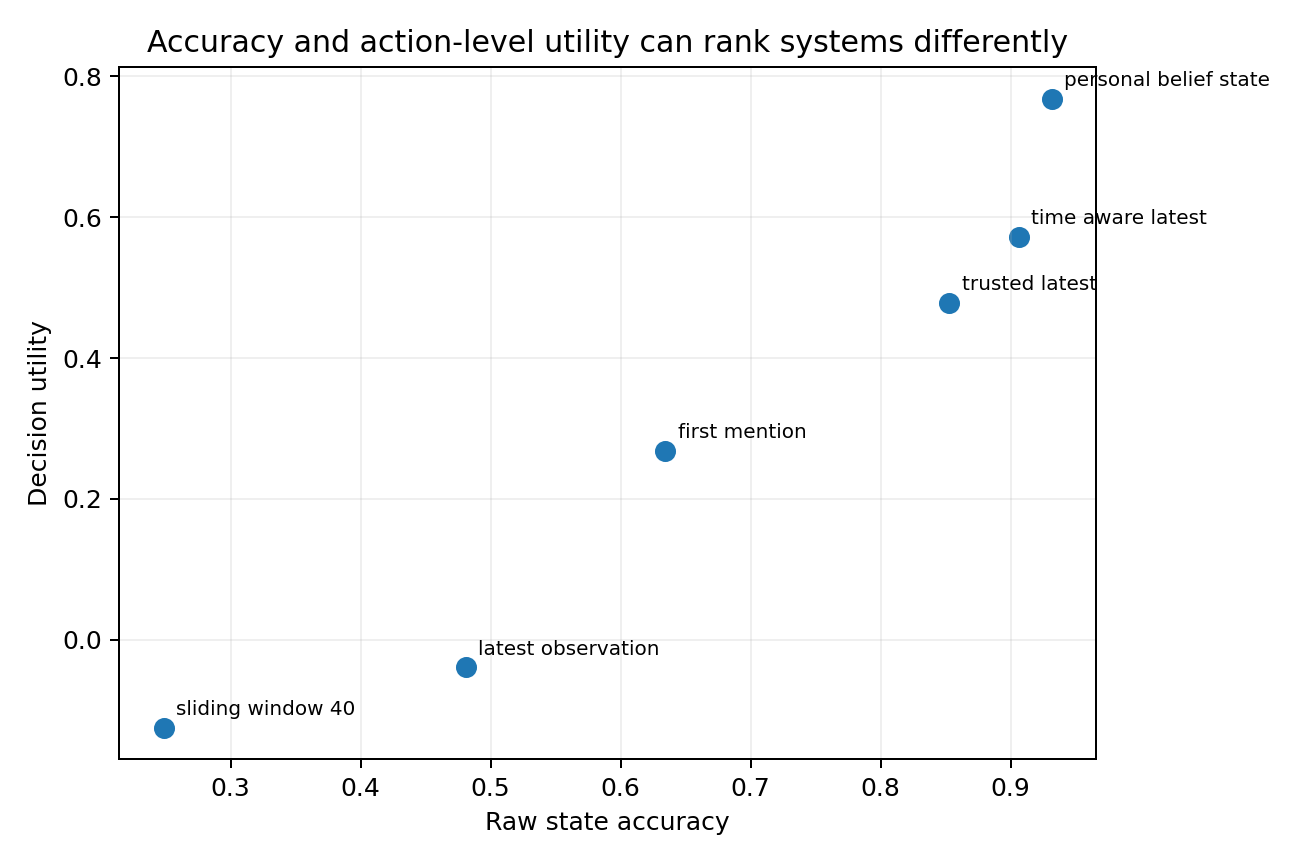
\includegraphics{paper/figures/accuracy_vs_utility.png}
\caption{Raw state accuracy and decision utility on the standard
controlled benchmark.}
\end{figure}

\subsubsection{7.2 Held-out standard
seeds}\label{held-out-standard-seeds}

PBS hyperparameters are frozen from development seeds 1--3. Across test
seeds 10--19, relative to time-aware-latest:

\begin{longtable}[]{@{}lrr@{}}
\toprule\noalign{}
PBS − time-aware-latest & Mean & 95\% bootstrap interval \\
\midrule\noalign{}
\endhead
\bottomrule\noalign{}
\endlastfoot
Decision utility & \textbf{+0.210} & \textbf{{[}+0.205, +0.216{]}} \\
State accuracy & \textbf{+0.024} & \textbf{{[}+0.021, +0.026{]}} \\
Selective accuracy & −0.020 & {[}−0.022, −0.018{]} \\
Brier reduction & \textbf{+0.020} & \textbf{{[}+0.019, +0.021{]}} \\
\end{longtable}

The selective-accuracy decrease is expected: PBS deliberately covers
many more cases rather than only high-confidence explicit observations.

\subsubsection{7.3 Long-horizon native-confidence
diagnostic}\label{long-horizon-native-confidence-diagnostic}

With each tracker using its \textbf{native, unmatched confidence scale},
800-turn histories produce an apparent ranking disagreement. In the
checked-in shift run, time-aware-latest has slightly \textbf{higher} raw
state accuracy than PBS (0.844 vs.~0.831) but lower fixed-threshold
decision utility (0.207 vs.~0.503). Across ten held-out long-horizon
seeds:

\begin{longtable}[]{@{}
  >{\raggedright\arraybackslash}p{(\columnwidth - 4\tabcolsep) * \real{0.2727}}
  >{\raggedleft\arraybackslash}p{(\columnwidth - 4\tabcolsep) * \real{0.3636}}
  >{\raggedleft\arraybackslash}p{(\columnwidth - 4\tabcolsep) * \real{0.3636}}@{}}
\toprule\noalign{}
\begin{minipage}[b]{\linewidth}\raggedright
PBS − time-aware-latest
\end{minipage} & \begin{minipage}[b]{\linewidth}\raggedleft
Mean
\end{minipage} & \begin{minipage}[b]{\linewidth}\raggedleft
95\% bootstrap interval
\end{minipage} \\
\midrule\noalign{}
\endhead
\bottomrule\noalign{}
\endlastfoot
State accuracy & \textbf{−0.014} & \textbf{{[}−0.017, −0.012{]}} \\
Native-confidence decision utility & \textbf{+0.284} &
\textbf{{[}+0.276, +0.291{]}} \\
Coverage & \textbf{+0.328} & \textbf{{[}+0.322, +0.333{]}} \\
Brier reduction & \textbf{+0.016} & \textbf{{[}+0.014, +0.017{]}} \\
\end{longtable}

This comparison is intentionally treated as a \textbf{diagnostic, not a
fair model-selection result}, because the systems' confidence scales
have not yet been equalized. Section 7.6 applies the same
development-only calibration opportunity to every tracker and shows that
the fixed-threshold utility ordering reverses. The stable conclusion is
therefore about protocol sensitivity, not a universal PBS utility
advantage.

\begin{figure}
\centering
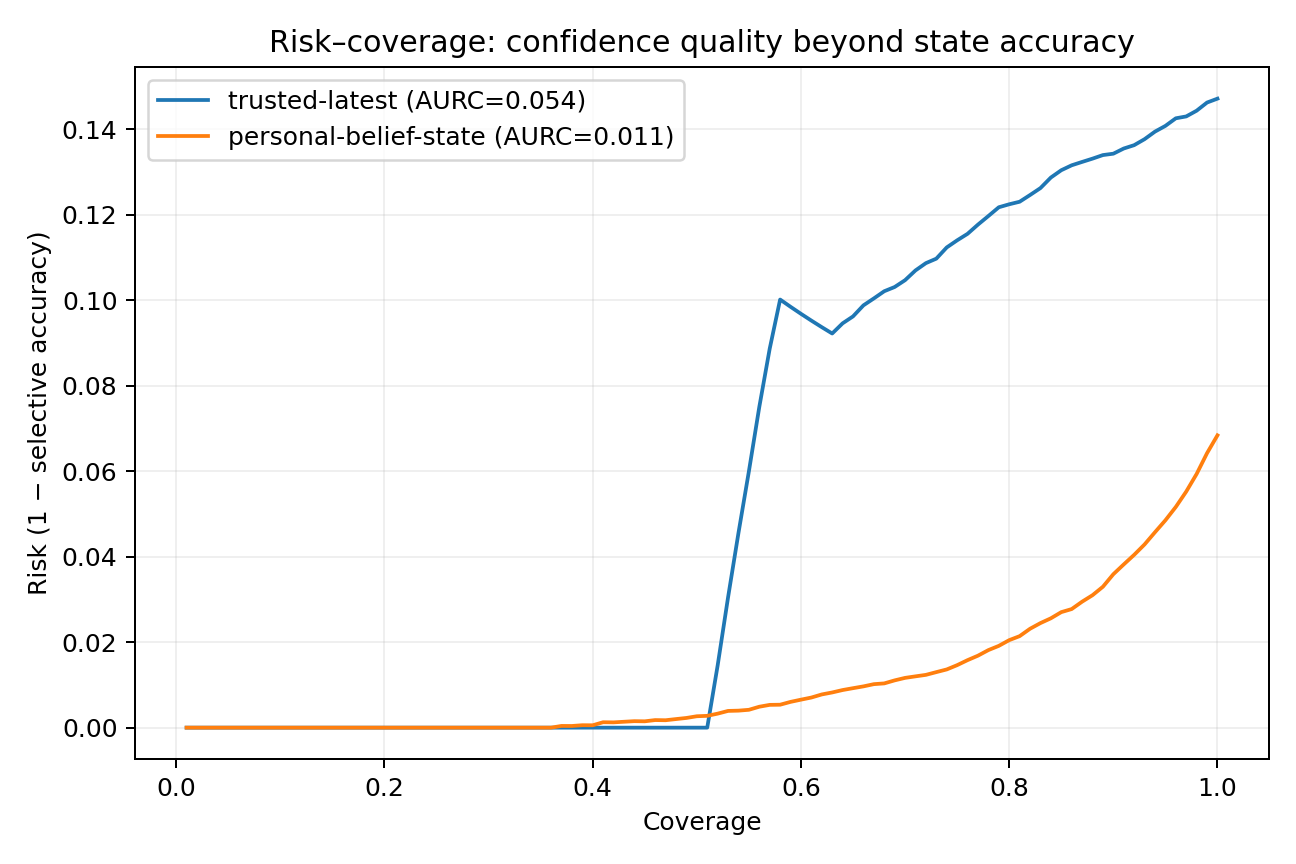
\includegraphics{paper/figures/risk_coverage.png}
\caption{Risk--coverage curve for the strongest controlled systems.}
\end{figure}

\subsubsection{7.4 Distribution shifts}\label{distribution-shifts-1}

PBS has the highest checked-in decision utility in all five regimes. Its
utility remains 0.736 under high noise, 0.705 under implicit-heavy
histories, 0.773 under temporary-heavy histories, and 0.503 at 800
turns.

\begin{figure}
\centering
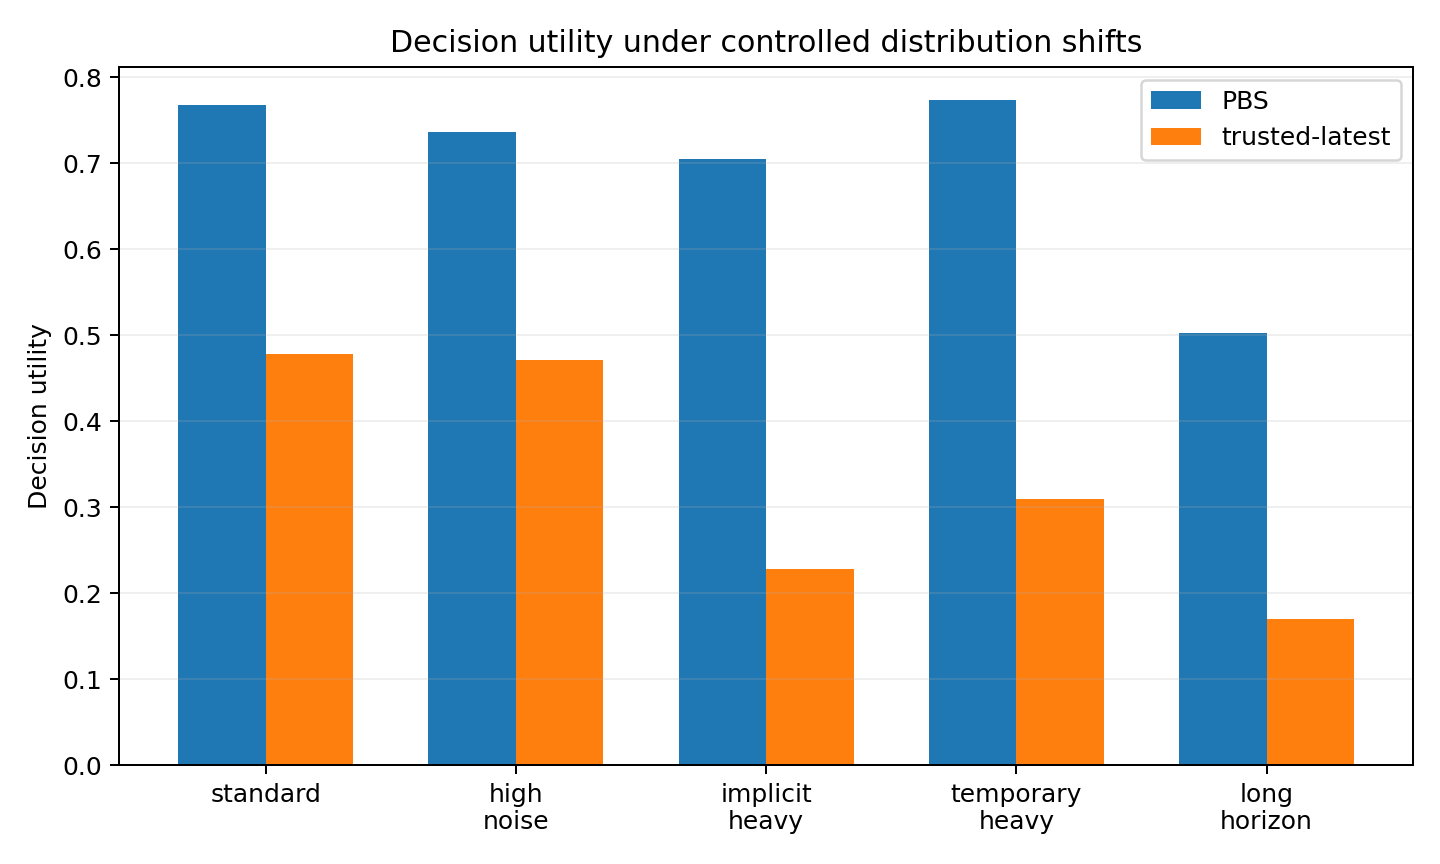
\includegraphics{paper/figures/distribution_shifts.png}
\caption{Decision utility under controlled distribution shifts.}
\end{figure}

\subsubsection{7.5 Additional robustness
analyses}\label{additional-robustness-analyses}

Sensitivity sweeps, component ablations, a 48-cell stress grid, and
exact paired tests are reported in the technical appendix and released
artifacts. Briefly, PBS is preferred to time-aware-latest in
\textbf{23/30} threshold/cost cells before shared calibration;
provenance reliability and evidence aggregation are the largest PBS
ablation effects; and PBS has higher utility in \textbf{46/48}
controlled stress cells but is not uniformly superior. These analyses
narrow rather than broaden the claim: operating-point conclusions depend
on calibration and cost assumptions, while mechanism effects are
generator-dependent. A supplementary trajectory-level agent-evaluation
extension also tests whether graders distinguish successful final states
from policy-compliant, verified trajectories; it is reported in Appendix
G and is not used as a frontier-model capability claim. Appendix I
further evaluates the frozen grader on five held-out attack families,
and Appendix J adds paired counterfactual checks of belief-state
robustness versus adaptivity.

\subsubsection{7.6 Equal-opportunity confidence calibration changes the
conclusion}\label{equal-opportunity-confidence-calibration-changes-the-conclusion}

A fixed action threshold is only comparable when confidence scales are
comparable. We therefore fit the same deliberately low-capacity post-hoc
calibrator for \textbf{every tracker} on development seeds 1--3 only:
each raw-confidence bucket is mapped to Laplace-smoothed empirical
correctness, then frozen for held-out evaluation. No test labels are
used.

On 800-turn held-out seeds, this changes the conclusion. The calibrated
time-aware-latest baseline obtains \textbf{0.687 decision utility},
compared with \textbf{0.588 for PBS}. PBS still has higher selective
accuracy (\textbf{0.908 vs.~0.844}) and slightly lower Brier
(\textbf{0.119 vs.~0.122}), but its lower coverage (\textbf{0.750
vs.~1.000}) is penalized at the chosen deferral cost. Thus the earlier
native-confidence utility advantage (\textbf{+0.284} on average) is not
protocol-invariant; after shared calibration the sign reverses to
approximately \textbf{−0.099}.

This is a central negative result. It does \textbf{not} imply that
time-aware-latest is globally better, nor that PBS is globally better.
It implies that fixed-threshold utility combines three
choices---confidence scale, action threshold, and deferral cost---and
can therefore change system ordering when those choices change. AURC is
less exposed to this particular confound because monotone post-hoc
calibration does not alter confidence ordering; in the checked-in
benchmark AURC remains \textbf{0.0107 for PBS vs.~0.0208 for
time-aware-latest}.

We therefore recommend a reporting hierarchy: (1) state accuracy, (2)
calibration error, (3) risk--coverage/AURC, and (4) operating-point
utility only after an explicitly shared calibration protocol. The
complete mappings and held-out results are released in
\texttt{reports/CALIBRATED\_BASELINES.md} and
\texttt{reports/CALIBRATION\_PROTOCOL\_ANALYSIS.md}.

A broader frozen protocol sweep reaches the same conclusion without
relying on a single threshold or calibrator. The focused
PBS-vs-time-aware slice reverses frequently across 75 cells, and the
full audit ranks \textbf{all six released baselines} under the same
protocol family. Time-aware-latest wins 45 cells, PBS 27, and
first-mention 3. Across unordered pairs of protocol cells, the
probability of selecting a different winner is \textbf{0.516}; mean
complete-ranking Kendall \(\tau\) is \textbf{0.699}, with a minimum of
\textbf{0.20}. To test whether this headline is a seed or grid artifact,
a separate 10-user-per-seed diagnostic runs \textbf{2,000 paired seed
bootstraps}, yielding winner-change probability \textbf{0.516 {[}0.507,
0.538{]}} and mean Kendall \(\tau\) \textbf{0.702 {[}0.692, 0.720{]}}.
Thirteen leave-one-level-out grid perturbations all retain multiple
winners; winner-change probability ranges \textbf{0.327--0.564}.
Appendix K reports the focused matrix, Appendix L the full-leaderboard
and benchmark-health audit, and Appendix M the seed/grid robustness
checks. These intervals quantify synthetic-generator seed variation
only; they are not population estimates or external leaderboard results.

\subsection{8. Relation to prior work}\label{relation-to-prior-work}

The personalization benchmark landscape is now crowded, so
PersonaMetrica does \textbf{not} claim to introduce the first benchmark
for preference following, evolving preferences, personalized memory, or
proactive assistance. PrefEval evaluates explicit and implicit
preference following in long-context conversations
\citep{zhao2025prefeval}. PersonaLens evaluates personalized
task-oriented assistants with simulated users and LLM judges
\citep{zhao2025personalens}. HorizonBench directly studies evolving
preferences over six-month synthetic histories and diagnoses
stale-belief failures \citep{li2026horizonbench}. BeliefShift evaluates
temporal belief consistency, contradiction resolution, and
evidence-driven revision \citep{myakala2026beliefshift}. PERMA models
event-driven preference evolution in realistic task environments
\citep{perma2026}. PerMemBench studies personalized memory-storage
policies \citep{in2026permem}, while PAHF studies continual
personalization with pre-action clarification and post-action feedback
\citep{liang2026pahf}. pi-Bench evaluates proactive personal assistants
with hidden intents, tools, and persistent sessions
\citep{zhang2026pibench}. OP-Bench targets over-personalization such as
irrelevance, repetition, and sycophancy \citep{hu2026opbench}.

PersonaMetrica targets a different layer: \textbf{measurement validity
when personalization systems emit confidence and that confidence gates
action}. Its core empirical object is not a new memory leaderboard but
\emph{ranking stability under defensible evaluation changes}.
Native-confidence utility and shared-calibration utility can select
different systems at the same nominal action threshold, while
threshold-free risk--coverage tells a different story again. The
trajectory extension then applies the same skepticism to the evaluator:
a grader that is perfect on authored perturbations can fail
catastrophically on held-out attack families, motivating causal-contract
checks, \texttt{Unknown} under missing evidence, grader fingerprints,
and disagreement review.

This positioning is deliberately narrower than a ``first'' claim.
Related work in selective prediction already establishes risk--coverage
and abstention as general evaluation tools, while 2026 work studies
ranking instability under prompt/evaluator variation
\citep{du2026promptstability, mahmood2026rankreversal},
disagreement-aware stable aggregation \citep{bonagiri2026stableval},
long-horizon trajectory attribution
\citep{chen2026trajectoryattribution}, and trajectory-level safety
calibration under adaptive attacks \citep{asif2026blindspot}.
PersonaMetrica therefore does \textbf{not} claim that rank instability,
trajectory attacks, or grader auditing are individually new. Its
narrower contribution is to connect protocol-sensitive system selection
with \textbf{evolving personal state}, confidence-gated action,
counterfactual preference interventions, and evaluator validity in one
reproducible artifact.

\subsection{9. Human and model evaluation
protocol}\label{human-and-model-evaluation-protocol}

The release contains \textbf{620 independently labelable tasks} (300
proactivity decisions, 320 belief-update decisions) with a browser
interface that hides simulator reference labels, plus a provider-neutral
external-model evaluator reporting accuracy, Brier, and ECE. It also
includes an executable adapter for the official HorizonBench per-item
result JSONL contract; the checked-in adapter run uses synthetic schema
fixtures only. These are \textbf{unexecuted external-evidence
infrastructure}: no human or frontier-model result is reported. The
intended next study holds the evaluation protocol fixed while replacing
simulator-derived evidence or labels with independent human/model
outputs.

\subsection{10. Limitations}\label{limitations}

PersonaMetrica-Bench begins \textbf{after structured evidence
extraction}, uses synthetic users, binary preference domains, designed
source reliabilities, and generator-defined transition processes. PBS
parameters are selected on development simulator seeds and should not be
interpreted as learned human preference dynamics. The benchmark can
exhibit generator--method coupling, and multilingual tags are metadata
rather than multilingual understanding results. No frontier-model table
or human-subject study is reported. Decision utility is task-dependent,
and this paper directly shows that its ranking can reverse after shared
confidence calibration; utility must therefore be interpreted only with
calibration, threshold, and deferral cost specified. Finally, the
current Croissant metadata and anonymous bundle are complete locally,
but venue-compliant external anonymous hosting remains a submission
requirement.

\subsection{11. Reproducibility and responsible
release}\label{reproducibility-and-responsible-release}

All controlled primary experiments run on CPU; the release records
seeds, generated data, scripts, figures, compute measurements, integrity
audits, a dataset card, Croissant metadata, and an anonymous submission
bundle. The benchmark contains only synthetic users. Because
personal-state systems can enable persistent profiling or overconfident
action, the broader system artifact includes forgetting, privacy-policy
hooks, permission boundaries, provenance, and outcome verification. No
human-subject result supports the present claims.

The practical evaluation implication is simple: when personal state can
trigger action, report \textbf{state accuracy, calibration,
risk--coverage/AURC, and any operating-point utility together}, and
apply a shared confidence calibration protocol before comparing
fixed-threshold action policies.

\subsection{12. Conclusion}\label{conclusion}

Personalization is a belief-update problem before it is a retrieval
problem, and an action problem after it. PersonaMetrica-Bench shows that
system rankings can change not only when moving from state accuracy to
action metrics, but also when the \textbf{confidence calibration and
action protocol itself} changes. In the controlled long-horizon setting,
native-confidence utility favors PBS, whereas equal development-only
post-hoc calibration can favor time-aware-latest at the same operating
point; threshold-free AURC still favors PBS. Across the full six-system
75-cell audit, even the leaderboard winner and complete ordering vary
substantially. The larger contribution is therefore evaluative rather
than algorithmic: long-horizon personal assistants should be compared
with explicit calibration protocols, threshold-free risk metrics, and
ranking-stability diagnostics rather than a single operating-point
leaderboard. PBS is one transparent reference implementation for
studying those interactions, not a claim of a universally superior
memory architecture.
